\chapter{Clustering}
\minitoc
\thispagestyle{empty}
\newpage

\section{Introduction}
Le clustering est un moyen de classer les données brutes de manière raisonnable et recherche les modèles cachés qui peuvent exister dans les ensembles de données [21].
Le clustering est une méthode de l’apprentissage automatique non-supervisé et un outil mathématique qui tente de découvrir des structures ou certains modèles dans un jeu de données, où les objets à l'intérieur de chaque cluster montrent un certain degré de similitude [2]. Le but de l'analyse de cluster consiste à partitionner un ensemble de N objets en clusters de sorte que les objets dans le cluster doivent être similaires les uns aux autres et les objets dans différents groupes doivent être différents avec les uns des autres [3]. Il peut être réalisé par divers algorithmes qui diffèrent considérablement dans leur notion de ce qui constitue un cluster et comment les trouver efficacement. L'analyse de cluster est un processus itératif de découverte de connaissances ou d'optimisation multi-objectifs interactive [2]. Les chercheurs ont mis au point de nombreux algorithmes de clustering, qui ont été largement appliqués. Ils peuvent être globalement classés en deux groupes : partitionnelle et hiérarchique. Les algorithmes de partition traitent les données d'entrée et créent une partition qui regroupe les données en clusters. En revanche, les algorithmes hiérarchiques créent un ensemble de partitions imbriquées appelé hiérarchie de cluster [6]. En général, un algorithme de clustering hiérarchique partitionne un ensemble de données en différents clusters via un agglomératif ou une approche de division basée sur un dendrogramme [5].
Les notions populaires du clustering incluent des groupes avec de petites distances entre les membres du cluster, des zones denses de l’espace de données, des intervalles ou des distributions statiques particulières [il faut reformuler la phrase]. \\

Le clustering est une méthode qui cherche à minimiser l’inertie intra-cluster et maximiser l’inertie inter-cluster.Pour minimiser l’inertie intra-cluster et maximiser l’inertie inter-cluster, les algorithmes de clustering utilise des métriques pour mesurer la distance entre les clusters et les critères de liaison qui sont la façon dont la distance entre les clusters est calculée. \\

Avant de rentrer directement sur le fonctionnement des algorithmes de clustering, nous verrons d’abord les métriques et les critères de liaison qui sont utiliser dans le processus du clustering.

\section{Les métriques}
Le choix d'une métrique appropriée influencera la forme des grappes, car certains éléments peuvent être relativement plus proches les uns des autres sous une métrique que dans une autre. \\
Par exemple, en deux dimensions, sous la métrique de distance Manhattan, la distance entre l'origine (0,0) et (.5, .5) est la même que la distance entre l'origine et (0, 1), tandis que sous le distance euclidienne métrique, cette dernière est strictement supérieure. \\
Certaines métriques couramment utilisées pour le clustering hiérarchique sont :

\begin{table}[!htbp]
    \centering
	\begin{tabular}{|c| c|}%\(\displaystyle \)
	\hline
	 \textbf{Names} & \textbf{Formula}  \\ \hline
	 Euclidean  & \(\displaystyle \left\lVert a - b\right\rVert_{2} = \sqrt{\sum_{i}^{} (a_{i} - b_{i})^{2} } \)   \\  \hline
	 Squared Euclidean distance  & \(\displaystyle \left\lVert a - b\right\rVert_{2}^{2} = \sum_{i}^{} (a_{i} - b_{i})^{2} \)   \\  \hline
	 Manhattan distance  & \(\displaystyle \left\lVert a - b\right\rVert_{1} = \sum_{i}^{} \left\lvert a_{i} - b_{i} \right\rvert \)   \\  \hline
	 Maximum distance  & \(\displaystyle \left\lVert a - b\right\rVert_{\infty} = \max_{i} \left\lvert a_{i} - b_{i} \right\rvert  \)   \\  \hline
	 Mahalanobis distance  & \(\displaystyle \sqrt{(a-b)^{T}S^{-1}(a-b)} \) where S is the Covariance matrix   \\  \hline
	\end{tabular}
	\caption{Les métriques }
	\label{metrics}
\end{table}

\section{Critère de liaison}
Le critère de liaison détermine la distance entre les ensembles d'observations en fonction des distances par paires entre observations. \\
Certains critères de liaison couramment utilisés entre deux ensembles de les observations A et B sont :

\begin{table}[!htbp]
    \centering
	\begin{tabular}{|c| c|}
	\hline
	 \textbf{Names} & \textbf{Formula}  \\ \hline
	 \makecell{Maximum or \\ complete-linkage clustering}   & \(\displaystyle \max \{d(a,b): a \in A,b \in B \} \)   \\  \hline
	 \makecell{Minimum or \\ single-linkage clustering}   & \(\displaystyle \min \{d(a,b): a \in A,b \in B \} \)   \\  \hline
	 \makecell{ Unweighted average linkage \\ clustering (or \textbf{UPGMA})} & \(\displaystyle \frac{1}{ \left\lvert A\right\rvert  \cdot \left\lvert B\right\rvert } \sum_{a \in A} \sum_{b \in B} d(a,b)  \)   \\  \hline
	 \makecell{Weighted average linkage \\ clustering (or \textbf{WPGMA})}  & \(\displaystyle d(i \cup j,k) = \frac{d(i,k)+d(j,k)}{2} \)   \\  \hline
	 \makecell{Centroid linkage clustering,\\ or \textbf{UPGMC}}   & \makecell{\(\displaystyle \left\lVert c_{s} - c_{t} \right\rVert \) where \(\displaystyle c_{s} \) and \(\displaystyle c_{t} \)  are the \\ centroids of clusters  \(\displaystyle s \) and \(\displaystyle t \), respectively.}   \\  \hline
	  Minimum energy clustering  & \(\displaystyle \frac{2}{nm}\sum_{i,j=1}^{n,m} \left\lVert
	  a_{i} - b_{j}\right\rVert^{2} - \frac{1}{n^{2}} \sum_{i,j=1}^{n} \left\lVert
	  a_{i} - a_{j}\right\rVert^{2}  - \frac{1}{m^{2}} \sum_{i,j=1}^{m} \left\lVert
	  b_{i} - b_{j}\right\rVert^{2}   \)   \\  \hline
	\end{tabular}
	\caption{Les critères de liaison }
	\label{linkage_criteria}
\end{table}

Le clustering est une méthode qui cherche à minimiser l’inertie intra-cluster et maximiser l’inertie inter-cluster. Il existe donc deux types de distance, celle entre les objets des différents clusters qui est la distance inter-cluster et celle entre les objets du même cluster qui est la distance intra-cluster.

\begin{figure}[H]
	\begin{center}
		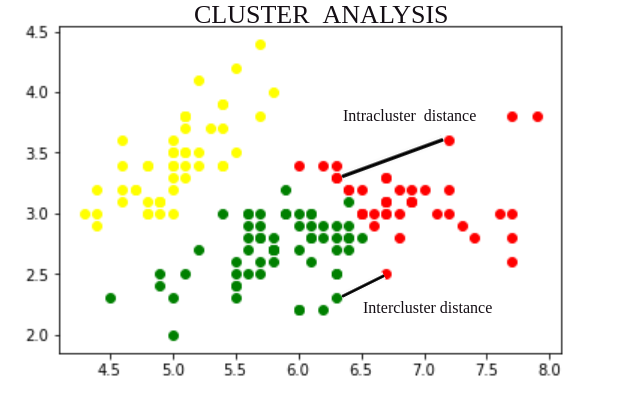
\includegraphics[width=\textwidth]{images/chapitre6/inter-intra_clusters__distnce.png}
	\end{center}
\caption{Distances intracluster et intercluster.}
\label{inter_intra_clusters}
\end{figure}

\subsection{Distance inter-cluster}
La distance inter-cluster est la distance entre deux objets appartenant à deux clusters différents. Il y’a 5 types de distance inter-cluster :

\subsubsection{Distance de liaison unique}
La distance de liaison unique est la distance la plus proche entre deux objets appartenant à deux clusters différents. Le clustering de liaison unique est basé sur le critère de connectivité. La distances entre deux clusters p et q est [13] :

 
\begin{equation}
     \delta (S,T) = \min  \Bigg\{
\begin{tabular}{@{}l@{}}
    \(\displaystyle d(x,y) \)  \\
    \(\displaystyle x \in S,y \in T \) 
\end{tabular} \Bigg\}
\end{equation}

Le principal avantage de la liaison simple est qu'elle peut gérer des formes non elliptiques [11] [NR]. Cependant, il est sensible au bruit et aux valeurs aberrantes [10] [12].

\subsubsection{Distance de liaison complète}
La distance de liaison complète est la distance entre deux objets les plus éloignés appartenant à deux groupes différents. Le regroupement de liens complet est également appelé la méthode la plus éloignée. Il utilise la plus grande distance entre les points de données dans deux clusters p et q comme :

\begin{equation}
	\delta (S,T) = \max  \Bigg\{
\begin{tabular}{@{}l@{}}
   \(\displaystyle d(x,y) \)  \\
   \(\displaystyle x \in S,y \in T \) 
\end{tabular} \Bigg\}
\end{equation}

Il ne tient pas compte de la structure du cluster. Il ne peut pas détecter les amas non sphériques [11] [NR].

\subsubsection{Distance de liaison moyenne}
La distance de liaison moyenne est la distance moyenne entre tous les objets appartenant à deux groupes différents. Le clustering de liaison moyenne a une procédure similaire comme liaison unique sauf le calcul de la distance entre deux clusters. Il utilise la moyenne des paires distance entre les points de deux clusters p et q comme [11] :
\begin{equation}
	\begin{split}
		\delta (S,T) = \frac{1}{\left\lvert S \right\rvert \left\lvert T \right\rvert  } \sum_{_{ x \in S},_{y \in T}} d(x,y)  \\
	\end{split}
\end{equation}
Il est moins sensible au bruit et aux valeurs aberrantes. Le seul inconvénient est sa polarisation vers les amas globulaires [12].

\subsubsection{Centroïde Linkage Distance}
La distance de liaison centroïde est la distance entre les centres de contre et vt deux groupes S et T respectivement, définis comme :

\begin{equation}
	\begin{tabular}{@{}l@{}}
		\(\displaystyle \delta (S,T) = d(v_{s}, v_{t} ) \) où \\ \\
		\(\displaystyle v_{s} = \frac{1}{\left\lvert S \right\rvert}  \sum_{x \in S} x,v_{t} = \frac{1}{\left\lvert T \right\rvert} \sum_{y \in T}y  \) 
	\end{tabular} 
\end{equation}

\subsubsection{Distance de liaison moyenne du centre de gravité}
La distance de liaison moyenne du centre de gravité est la distance entre le centre d'un cluster et tous les objets appartenant à un autre cluster, définie comme :

\begin{equation}
	\delta (S,T) = \frac{1}{\left\lvert S \right\rvert  + \left\lvert T \right\rvert  }  \Bigg\{
\begin{tabular}{@{}l@{}}
   \(\displaystyle \sum_{x \in S} d(x,vt) + \sum_{y \in T}d(y,vs) \)
\end{tabular} \Bigg\}
\end{equation}

\subsection{Distance intra-cluster}
La distance intra-cluster est la distance entre deux objets appartenant au même cluster. Il y’en a 3 types :

\subsubsection{Distance de diamètre complet}
La distance de diamètre complet est la distance entre deux objets les plus éloignés appartenant au même cluster défini comme :

\begin{equation}
	\begin{split}
		\Delta (S) = \max_{x,y \in S} \{ d(x,y) \}  \\
	\end{split}
\end{equation}

\subsubsection{Distance de diamètre moyen}
La distance de diamètre moyen est la distance moyenne entre tous les objets appartenant au même cluster défini comme :

\begin{equation}
	\begin{split}
		\Delta (S) = \frac{1}{\left\lvert S \right\rvert \cdot  (\left\lvert S \right\rvert - 1)} \sum_{x,y \in S ; x \neq y} \{ d(x,y) \} \\
	\end{split}
\end{equation}

\subsubsection{Diamètre barycentre Distance}
La distance de diamètre barycentre est à double distance moyenne entre tous les objets et le centre de groupe de s défini comme :

\begin{equation}
	\Delta (S) = 2  \Bigg \{
	\frac{\sum_{x \in S}d(x,\overline{v})}{\left\lvert S \right\rvert } \Bigg\} 
	\hspace{20pt} où \hspace{10pt} \overline{v} = \frac{1}{\left\lvert S \right\rvert} \sum_{x \in S}x
\end{equation}

\section{Le clustering hiérarchique}
\subsection{Définition}
Dès les années 1970, on a estimé qu'environ 75\% de tous les travaux publiés sur le clustering utilisaient des algorithmes hiérarchiques [1]. Le clustering hiérarchique est une méthode de clustering qui permet d’identifier des clusters dans un ensemble de données. Contrairement aux autres méthodes de clustering comme le k-means, le clustering hiérarchique n’oblige pas à spécifier à l’avance le nombre de clusters à générer. Et le résultat est une représentation arborescente des observations, appelée dendrogramme. L'interprétation des informations contenues dans un dendrogramme est souvent d'un ou plusieurs types : relations d'inclusion d'ensemble, partition des ensembles d'objets et clusters significatifs [1]. C’est une méthode de clustering d’apprentissage automatique non supervisé qui procède à une décomposition de données en cherchant à construire une hiérarchie de clusters. Cette méthode suit deux approches basées sur la direction du progrès, c'est-à-dire s'il s'agit du flux descendant ou ascendant de création de clusters. Il s'agit respectivement de l'Approche Divisive et de l'Approche Agglomérative. \\
Le clustering agglomératif commence à partir des clusters singleton et obtient une hiérarchie en fusionnant successivement les clusters, tandis que le clustering divisif commence par un cluster unique contenant tous les points et se poursuit en fractionnant les clusters de manière itérative [7]. \\
Un algorithme de regroupement hiérarchique crée une décomposition hiérarchique de l'ensemble donné d'objets de données. Il peut être classé comme agglomératif ou diviseur. L'avantage du clustering hiérarchique est qu'il n'est pas déterminé par l'initialisation et les minima locaux. Les lacunes de la classification hiérarchique sont les suivantes : (1) elle n'est pas pratique pour les grands ensembles de données en raison de la complexité de calcul élevée ; (2) il n'intègre aucune connaissance a priori telle que les formes de grappes ; (3) le regroupement est statique, c'est-à-dire que les points de données d'un cluster au stade précoce ne peuvent pas se déplacer vers un autre cluster au dernier stade [9] [NR].

\subsection{Clustering hiérarchique agglomératif}
En clustering, l'un des algorithmes les plus largement utilisés est les algorithmes agglomératifs. Il s'agit d'une approche « ascendante » : chaque observation commence dans son propre cluster, et les paires de clusters sont fusionnées au fur et à mesure que l'on monte dans la hiérarchie. Les résultats de la classification hiérarchique sont généralement présentés dans un dendrogramme [2] [NR].
Cependant, pour certains cas particuliers, des méthodes agglomératives efficaces optimales (de complexité) sont connues : SLINK pour une liaison simple et CLINK pour un clustering à liaison complète [2] [NR].
L’algorithme de clustering AHC a trois mesures de distance principales : liaison unique, liaison complète et liaison moyenne [6] [NR].
L’algorithme AHC est également appelé cluster le plus proche voisin algorithme lorsque la mesure de couplage unique est utilisée pour distance entre les grappes [6] [NR].
Dans le clustering hiérarchique agglomératif classique, une paire de clusters à fusionner à la distance minimale inter-cluster [9] [NR].

\subsubsection{Exemple de clustering agglomératif}

Par exemple, supposons que les données ci-dessous doivent être regroupées et que la métrique de distance est la distance euclidienne.
\begin{figure}[H]
	\begin{center}
		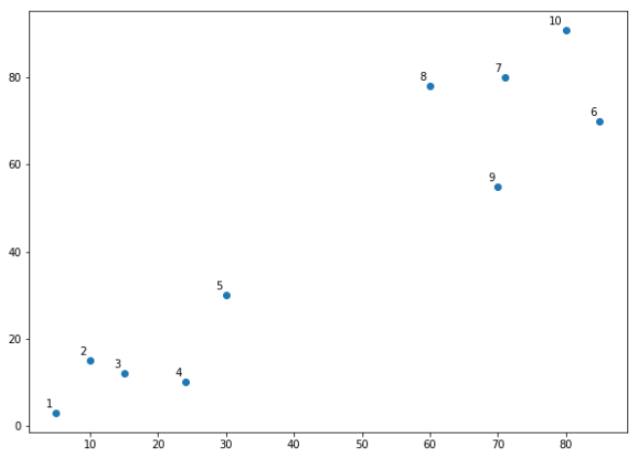
\includegraphics[width=\textwidth]{images/chapitre6/agglo_clustering.png}
	\end{center}
	\caption{Données en 2 dimensions}
	\label{agglo_clustering}
\end{figure}

Le dendrogramme obtenu après le clustering serait comme tel :
\begin{figure}[H]
	\begin{center}
		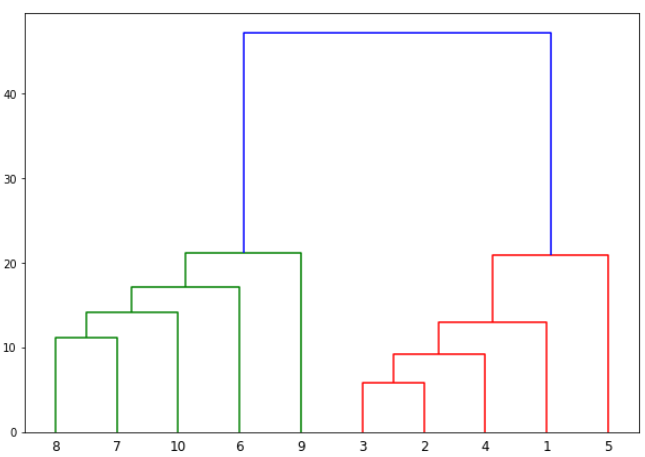
\includegraphics[width=\textwidth]{images/chapitre6/dendrogram.png}
	\end{center}
	\caption{Dendrogramme}
	\label{dendrogramme}
\end{figure}

Pour obtenir le nombre de clusters optimal avec le dendrogramme, la méthode la plus connue est celle qui cherche la distance verticale la plus élevée qui ne croise aucun cluster et les lignes verticales franchissent le seuil représente le nombre optimal de clusters. En utilisant le dendrogramme précédant on obtient 2 clusters comme le montre la figure ci-dessous.

\subsection{Clustering hiérarchique divisive}
Le principe de base du clustering divisif a été publié sous le nom d'algorithme DIANA (Divisive Analysis Clustering) [15]. Contrairement au clustering hiérarchique agglomératif, le clustering hiérarchique divisif suit une approche descendante dans laquelle tous les points de données appartiennent à un seul grand cluster et celui-ci est divisé en groupes plus petits en fonction d'une logique de terminaison ou d'un point au-delà duquel il n'y aura plus de division de points de données. Le principe du clustering divisif est illustrer par la figure ci-dessous. \\
Le fractionnement est effectué de manière récursive au fur et à mesure que l'on descend dans la hiérarchie et il existe (2n-1) -1  façons de diviser un ensemble de n objets en deux sous-ensembles [14]. Par conséquent le fractionnement prend top du temps sur la recherche de toutes les bipartitions possibles. Le clustering hiérarchique divisif procède par le fractionnement des clusters en deux clusters les moins similaires en utilisant des critères de type distance ou rapport et ensuite détermine les niveaux des nœuds (qui représente les groupes obtenus dans le dendrogramme).
\subsubsection{Procédures de fractionnement des clusters}
Un certain nombre de procédures de fractionnement ont été conçus dans le passé. La procédure de Williams Et Lambert (1959) [16] est dite monothéique dans le sens où les ensembles d'objets sont divisé en fonction des valeurs d'une seule variable. Cette idée a été mise à jour en utilisant une composante principale au lieu d'une seule variable (algorithme Principal Directions Divisive Partitioning ou PDDP par Boley 1997) [14]. \\
Une autre approche pour contourner la complexité du fractionnement consiste à extraire un ou plusieurs objets, de l'ensemble à fractionner. Macnaughton-Smith et al. (1964) [17] ont proposé de sélectionner le plus objet distant du cluster comme graine pour un nouveau cluster distinct. Puis ils s'agrègent à ceci amorce les objets qui sont plus proches du nouveau sous-ensemble que du reste du cluster actuel [14]. \\
Une idée similaire a été développée par Hubert (1973) [18], il a suggéré d'utiliser une paire d'objets comme germes de la nouvelle bipartition. Son choix a été de sélectionner les deux objets qui sont les plus dissemblables, puis de construire les deux sous-clusters en fonction des distances (ou fonction des distances) à ces graines [14]. \\
Exploitant cette idée, Roux [19][20] considérait bipartitions générées par toutes les paires d'objets, en conservant la bipartition avec la meilleure évaluation de certains critères a priori [14]. \\

\subsubsection{Evaluations des bipartitions}
Quel que soit le critère retenu, il faut noter qu’une série de très bonnes bipartitions ne se traduit pas automatiquement par une bonne hiérarchie.
Les critères qui permettent d’évaluer les bipartitions sont de deux types : critère de type distance et les critères de type rapport.

\subsubsection{Déterminations de niveaux de nœuds }
Pour l’algorithme agglomératif, la valeur du critère devient le niveau du nœud correspondant, et le dessin de l’arbre hiérarchique ne montre aucun croisement (ou inversion) des branches.
Malheureusement, les procédures qui divisent, en général, ne bénéficient pas de cette propriété, en raison du non-optimalité des fractionnements successifs. Une règle est alors nécessaire pour obtenir des niveaux cohérents et une véritable représentation arborescente.
\subsection{Conclusion}
\section{Le clustering partitionnel}

\subsection{K-means clustering}
K-means est un algorithme de clustering qui est largement utiliser pour analyser les clusters des grands ensembles de données. Il a été proposé par MacQueen en 1967 et c’était l’un des algorithmes d’apprentissage non supervisé le plus simple, qui a été appliqué pour résoudre les problèmes du clustering [22]. Il s'agit d'un algorithme de partitionnement des clusters, cette méthode consiste à classer les objets d’un jeu de donnés en k clusters différents, de telle sorte que les clusters générés sont compacts et indépendants [23].

\subsubsection{Le fonctionnement de l’algorithme k-means}
K-Means clustering fonctionne de cette façon : par exemple pour regrouper les données en trois clusters on commence par placer trois point appelé centroïde au hasard dans le jeu de données ensuite on affecte chaque point de data set au centroïde le plus proche ce qui nous donne trois clusters puis on déplace chaque centroïde au milieu de son cluster, on recommence jusqu’à ce que les centroïdes converge vers une position d’équilibre. L’algorithme requière donc à l’initialisation le nombre k de cluster à générer et k centroïdes (les centre des clusters) sont initialise avec des coordonnées aléatoires.

\subsubsection{Les étapes de l’algorithme}
L’algorithme de K-means clustering est un algorithme itératif qui procède comme suit :

\begin{itemize}
	\item	Sélection de k clusters a génère, où la valeur k est fixée à l'avance.
	\item	Initialisation des centroïdes avec de coordonnées aléatoires.
	\item	Calcul de la distance entre les objets et le centre de gravité du cluster.
	\item	Affectation des points au centroïde le plus proche.
	\item	Déplacement du centroïde à la moyenne du cluster.
	\item	Répétition des étapes précédente jusqu'à ce qu'il n'y ait pas de changement au centre des clusters.
\end{itemize}

Les étapes sont illustrées par la figure ci-dessous.

\begin{figure}[H]
	\begin{center}
		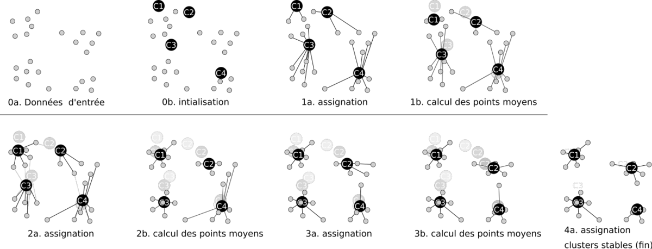
\includegraphics[width=\textwidth]{images/chapitre6/kmeans_steps.png}
	\end{center}
	\caption{Les étapes de l'algorithme k-means.}
	\label{kmeans_steps}
\end{figure}

Apres l’initialisation du nombre k des clusters a trouvées dans le jeu de données et k centroïdes, la distance euclidienne est généralement considérée pour déterminer la distance entre chaque objet de données et les centres du cluster. Cette distance est utilisée pour regrouper chaque objet de données au centre le plus proche [24]. La distance euclidienne entre un vecteur x = (x 1 , x 2 ,… x n ) et un autre vecteur y = (y 1 , y 2 ,… y n ), La distance euclidienne d (x i , y i ) peut être obtenue comme suit:
\begin{equation}
    d(x_{i}, y_{i}) = \left[\sum_{i=1}^{n}(x_{i} - y_{i})^{2} \right]^{\frac{1}{2}}
\end{equation}

Lorsque tous les objets de données sont inclus dans certains clusters, la première étape est terminée et un regroupement précoce est effectué. Ce processus itératif continue jusqu'à ce que la fonction de critère devienne le minimum [23]. \\
En supposant que l'objet cible est x, x i indique la moyenne du cluster C i, la fonction critère est définie comme suit :

\begin{equation}
    E = \sum_{i=1}^{k} \sum_{x \in C_{i}} \left\lvert x - x_{i} \right\rvert^{2}
\end{equation}

\subsubsection{Les lacunes de l’algorithme k-means}
L'algorithme de clustering k-means converge toujours vers le minimum local. Avant qu’il ne converge, l'algorithme doit calculer la distance entre chaque objet de données et chaque centre de cluster dans chaque itération. Du au choit aléatoire des centres de cluster initiaux, la valeur precise t connu sous le nom de nombre d'itérations k-means varie en fonction des centres de cluster de départ [25]. Aussi le fait de devoir choisir a priori le paramètre k est un inconvénient, car l’algorithme peut données des fausses informations sur les clusters générés et il est influencé par des valeurs aberrantes appelé aussi en anglais outliers.

\subsubsection{Les solutions aux lacunes de l’algorithme k-means}

Il n’est pas nécessaire de calculer la distance entre chaque objet de données et chaque centre de cluster dans chaque itération. En supposant que le cluster C s'est formé après le premier j itérations, l'objet de données x est affecté au cluster C, mais dans quelques itérations, l'objet de données x est toujours affecté au cluster C. Donc si on constate que la distance de l'objet de données x à chaque centre de cluster et constatez que la distance au cluster C  est la plus petite, il est possible d’arrêter le calcul de la distance lié l’objet x . 
Ceci que l’algorithme prend un long temps d'exécution affectant ainsi l'efficacité du clustering [23]. \\

Selon la position initiale des centroïdes, K-means peut donner de mauvais clusters. La configuration des clusters trouver par K-means peut ne pas être la plus optimale. On parle d’optimum local. La solution est d’exécuter K-means avec différentes positions de d´épart des centroïdes. La solution retenue est celle qui minimise la somme des distances entre les points(x) d’un cluster et son centre(u). Cela équivaut à minimiser la variance des clusters. K-means cherche la position des centroïdes qui minimise la distance entre les points
d’un cluster (Xi) et le centre (Ui) de ce dernier. Il cherche à minimise une fonction cout appeler Inertie et qui représente la distance entre le point d’un cluster et le centre de ce dernier. Les paramètres de la méthode kmeans() à optimiser pour le langage R :

\begin{itemize}
	\item  Centers : les clusters obtenus par l’algorithme son plus cohérant lorsque le nombre de centers demander par l’algorithme est le même que celui des clusters naturels du data set. Dans un data set avec de nombreuses dimensions il est difficile de voir un nombre de clusters à l’œil nu. Pour choisir le bon nombre de cluster il faut utiliser la méthode Elbow qui consiste à tracer l’évolution du cout du model en fonction du nombre de cluster et de détecter une zone de coude, cette zone nous indique le nombre de cluster optimale. C’est-`a-dire celui qui nous permet de réduire au maximum le cout du model tout en conservant un nombre raisonnable de cluster.
\end{itemize}

\begin{figure}[H]
	\begin{center}
		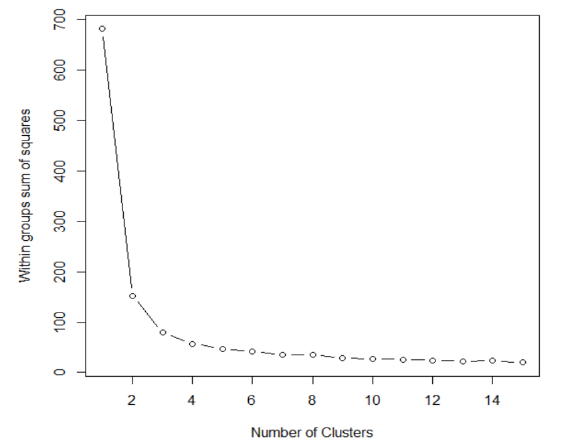
\includegraphics[width=\textwidth]{images/chapitre6/elbow_methods.png}
	\end{center}
	\caption{La méthode Elbow.}
	\label{elbow_methods}
\end{figure}

\begin{itemize}
	\item	nstart : avec le nombre donner au paramètre nstart l’algorithme tente plusieurs configuration initial de la position des centroïdes et retient la meilleurs configuration qui minimise la variance des cluster. La valeur par défaut est 1 mais la valeur recommander est 25 par contre cette valeur conduit `a un gaspillage de ressource avec un grand data set.
	\item	Iter.max : le nombre de fois que l’algorithme doit s’exécuter. La valeur par défaut est 10 ce qui permet au centroïdes de converger ver position d’équilibre.
	\item	algorithm : l’algorithme choisit est celui qui donne une plus forte cohérence des clusters. Avec python l’algorithme kmeans++ donne des meilleurs résultats.

\end{itemize}

\subsection{Fuzzy C-means}

\section{Indice de validité du clustering}

\section{Conclusion}

